\chapter{Methodology}

\section{Data Collection}
\paragraph{ }The data used in this study was collected from \ac{TIMBER} with the help of Dr. Gianluca Valentino who has access to the \acs{CERN} Intranet. Data was collected from the instrumentation discussed in Section \ref{sec::beam_instrumentation} and covers 1624 Injections over a time period of 3 months (from 17\textsuperscript{th} August to 20\textsuperscript{th} October 2018). During this time, approximately 65 experiments were performed.

\paragraph{ }The file sizes for the data gathered from each instrument ranged from 4 KB to 2 MB, these were initially individually analysed (refer to Section \ref{sec::Data_Cleaning_and_Analysis}) and then merged to create the dataset used to run the anomaly detection algorithms on (refer to Section \ref{sec::Merging_the_Dataset}). The total size of the merged datasets were 231 KB and 324 KB for Beam 1 and Beam 2 respectively. Loading this data in memory was not an issue since the file size is rather small, thus the problem of dealing with Big Data was not encountered in this study.

\section{Data Cleaning and Analysis}
\label{sec::Data_Cleaning_and_Analysis}
\paragraph{ }After Data Extraction, the provided datasets were analysed separately in order to understand their nature, remove any outliers and be able to aggregate the data correctly for further analysis. In this section the results of this analysis will be presented with the hopes that the reader will have a clearer understanding of later results. Note that all the steps mentioned here were repeated for both beams.

\subsection{\acs{TDI} \acs{BLM}s}
\paragraph{ }There are three \acs{BLM}s in the \acs{TDI}, each one giving 10 readings around the moment of injection. In order to get a total loss for each injection, the sum of each reading from the 3 monitors was taken (\ref{fig::TDI_BLM_hist}). From the plot of this data (Figure \ref{fig::Raw_TDI_BLM}) it was noted that at the exact moment of injection, there was a spike in the amount of beam lost. Thus, in order to then obtain a single reading corresponding to that particular injection, the maximum sum of losses for each 10 second window was kept. 

\begin{figure}[!t]
	\begin{minipage}[b]{0.475\linewidth}
		\centering
		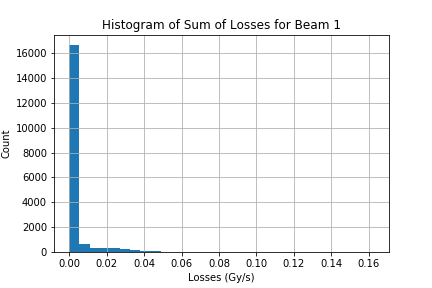
\includegraphics[width=\textwidth]{Histogram_of_Sum_of_Beam_Losses}
		\caption[BLM Histogram]{Histogram of Sum of Losses for Beam 1}
		\label{fig::TDI_BLM_hist}
	\end{minipage}	
	\hspace{0.25cm}
	\begin{minipage}[b]{0.475\linewidth}
		\centering
		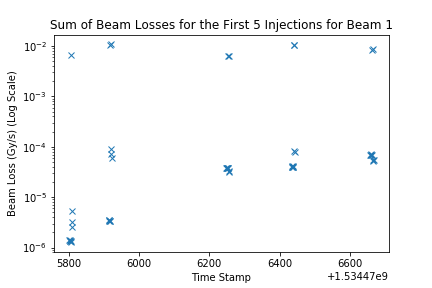
\includegraphics[width=\textwidth]{Raw_Beam_Loss}
		\caption[BLM Time Series]{Time Series of Beam Loss Sum for the First 5 Injections}
		\label{fig::Raw_TDI_BLM}
	\end{minipage}	
\end{figure}

\begin{figure}[b]
	\centering
	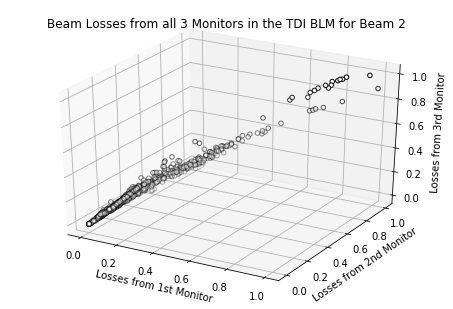
\includegraphics[width=0.6\textwidth]{BLM_3D_Plot}
	\caption[BLM Correlation Plot]{Beam Losses from all 3 Monitors in the TDI BLM for Beam 2 after MinMax Scaling}
	\label{fig::TDI_BLM_3D}
\end{figure}  

\paragraph{ }Once the relevant readings were kept, the sum column was dropped and this data set was saved to be used for anomaly detection. Furthermore, after scaling these points using MinMax scaling, it was noted from Figure \ref{fig::TDI_BLM_3D} that the readings from the 3 monitors are highly correlated. This was confirmed by computing the correlation matrix which gave a Pearson Correlation value $> 0.98$ for all pairwise comparisons.

\subsection{Abort Gap}
\paragraph{ }Similar to the \acs{TDI} \acs{BLM} readings, the Abort Gap readings also come in groups of 10 readings around the moment of injection. In this case however, the change in Abort Gap population is of interest for this study, thus the difference between every 10\textsuperscript{th} reading was kept and saved to be used for anomaly detection.

\begin{figure}[!t]
	\begin{minipage}[b]{0.475\linewidth}
		\centering
		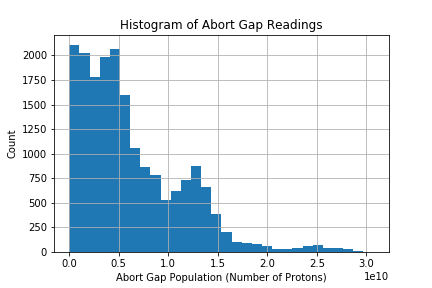
\includegraphics[width=\textwidth]{Histogram_of_Abort_Gap_Population}
		\caption[Abort Gap Histogram]{Histogram of Abort Gap Population for Beam 1}
		\label{fig::Abort_Gap_hist}
	\end{minipage}	
	\hspace{0.25cm}
	\begin{minipage}[b]{0.475\linewidth}
		\centering
		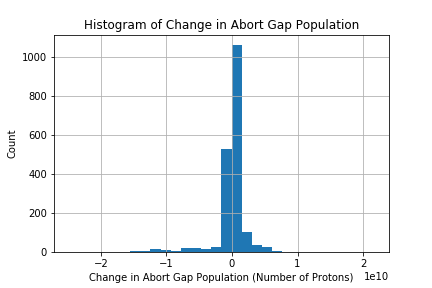
\includegraphics[width=\textwidth]{Histogram_of_Change_in_Abort_Gap_Population}
		\caption[Change in Abort Gap Histogram]{Histogram of Change in Abort Gap Population for Beam 1}
		\label{fig::Change_in_Abort_Gap_hist}
	\end{minipage}	
\end{figure}

\begin{figure}[b]
	\centering
	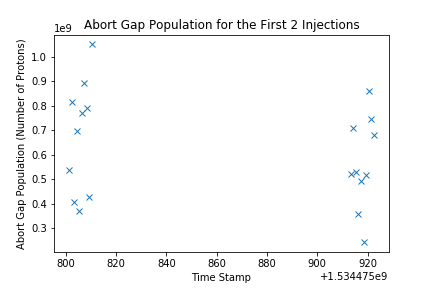
\includegraphics[width=0.6\textwidth]{Time_Series_of_Abort_Gap_Population}
	\caption[Abort Gap Time Series]{Time Series of Abort Gap  Population for the First 8 Injections}
	\label{fig::Abort_Gap_Time_Series}
\end{figure}  


\paragraph{ }Figures \ref{fig::Abort_Gap_hist} and \ref{fig::Change_in_Abort_Gap_hist} show the histograms of the Abort Gap Population and the Change in Abort Gap Population respectively. A time series plot of the Abort Gap Readings can be seen in Figure \ref{fig::Abort_Gap_Time_Series}.

\subsection{\acs{SPS} and \acs{LHC} Intensities}
\paragraph{ }As mentioned in Section \ref{sec::beam_instrumentation}, the raw \acs{LHC} intensity readings come in 10 readings around the moment of injection, while the \acs{SPS} intensity readings give the value of the beam intensity as its leaving the SPS. Thus, it is expected that change in \acs{LHC} intensity at the moment of injection (10\textsuperscript{th} reading - 1\textsuperscript{st} reading) should be approximately equal to the \acs{SPS} intensity value. Some of the beam however is lost in the transfer line (which is picked up by the \acs{TL} \acs{BLM}s) and as it enters the \acs{LHC} (which is picked up by the \acs{TDI} \acs{BLM}s). Thus as an input parameter to the anomaly detection algorithm, the change in \acs{LHC} intensities and the \acs{SPS} intensities were extracted for each injection and saved.

\begin{figure}[!t]
	\begin{minipage}[b]{0.475\linewidth}
		\centering
		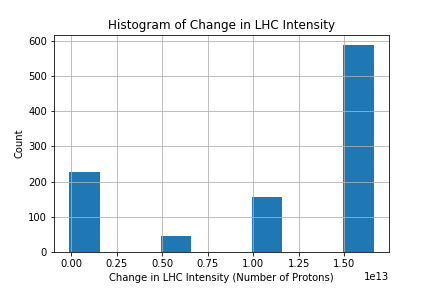
\includegraphics[width=\textwidth]{Histogram_of_Change_in_LHC_Intensity}
		\caption[LHC Intensity Histogram]{Histogram of Change in LHC Intensities for Beam 1}
		\label{fig::LHC_Intensity_hist}
	\end{minipage}	
	\hspace{0.25cm}
	\begin{minipage}[b]{0.475\linewidth}
		\centering
		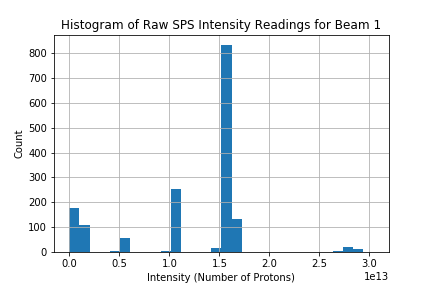
\includegraphics[width=\textwidth]{Histogram_of_SPS_Intensity}
		\caption[SPS Intensity Histogram]{Histogram of SPS Intensities for Beam 1}
		\label{fig::SPS_Intensity_hist}
	\end{minipage}	
\end{figure}

\begin{figure}[t]
	\centering
	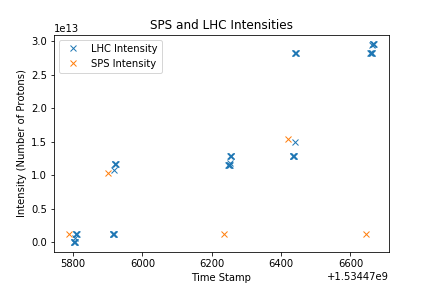
\includegraphics[width=0.6\textwidth]{SPS_and_LHC_Intensities}
	\caption[SPS and LHC Intensities]{Time Series of SPS and LHC Intensities for the first 5 Injections for Beam 1}
	\label{fig::SPS_and_LHC}
\end{figure} 

\paragraph{ }The histograms of the change in \acs{LHC} intensities and \acs{SPS} intensities can be seen in Figures \ref{fig::LHC_Intensity_hist} and \ref{fig::SPS_Intensity_hist} respectively. Figure \ref{fig::SPS_and_LHC} shows the increase in the \acs{LHC} reading and the corresponding \acs{SPS} intensity.

\subsection{\acs{TL} \acs{BLM}s}
\paragraph{ }Each \acs{TL} has 61 \acs{BLM}s each recording the amount of losses separately. The issue with these readings however is that their readings are not consistently stored after the experiments have been performed. In fact, during the time of the study, 13 of these monitors didn't have any logged data at all. The data which was logged was either 0 or close to 0. Thus, it was decided to drop this feature from the study.   

\subsection{\acs{TL} \acs{BPM}s}
\paragraph{ }There are 18 \acs{BPM}s in each \acs{TL}, each one giving a separate reading of the beam's deviation from its expected path at a different position in the \acs{TL}. From data taken from 1624 injections, data corresponding to 1420 injections was left for Beam 1 after removing all missing values and 1455 injections for Beam 2. Figure \ref{fig::BPM_hist} shows the histogram of the readings recorded by the first monitor in TI1.

\begin{figure}[b]
	\centering
	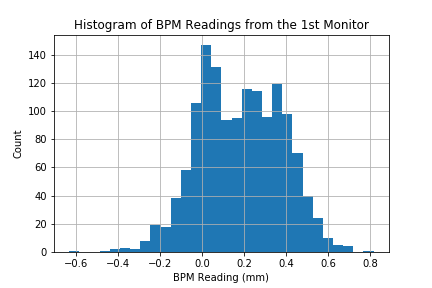
\includegraphics[width=0.6\textwidth]{Histogram_of_BPM}
	\caption[BPM Histogram]{Histogram of the readings recorded by the first monitor in TI1}
	\label{fig::BPM_hist}
\end{figure} 

\paragraph{ }In order to measure the beam drift over time, the first injection was assumed to be the expected path and the \acs{MSE} of each injection from the first injection was taken. This was worked out by taking the average of the squared differences in the readings of each monitor for each injection. This led to an interesting result which is presented in Chapter \ref{chp4}.

\subsection{Number of Bunches}
\paragraph{ }The number of bunches injected into the \acs{LHC} was another useful feature that needed to be extracted for normalisation. The beam losses, change in intensities and change in abort gap population are all relative to the number of bunches injected into the \acs{LHC} as for example, a large loss may only appear to be large because more bunches were injected into the LHC for that injection than previous injections. In this case, that large loss should not be considered an anomaly. 

\begin{figure}[t]
	\centering
	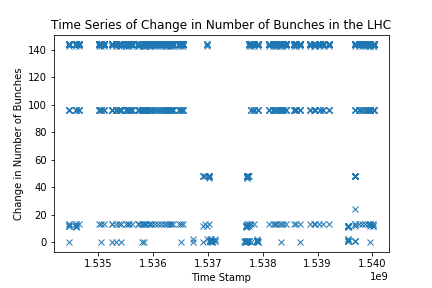
\includegraphics[width=0.6\textwidth]{Number_of_Bunches}
	\caption[Number of Bunches]{Number of Bunches Injected into the LHC for Beam 1}
	\label{fig::Number_of_Bunches}
\end{figure} 

\paragraph{ }The number of bunches circulating the \acs{LHC} was hence extracted around the time of each injection and the change in number of bunches was then worked out. Figure \ref{fig::Number_of_Bunches} shows the nature of this data and should give the reader an idea of how many bunches are injected at one time.

\section{Feature Selection}


\section{Merging the Dataset}
\label{sec::Merging_the_Dataset}